
\documentclass[12pt,a4paper,final]{article}
\usepackage[utf8]{inputenc}
\usepackage[francais]{babel}
\usepackage[T1]{fontenc}
\usepackage{amsmath}
\usepackage{amsfonts}
\usepackage{amsthm}
\usepackage{color}
\usepackage{amssymb}
\usepackage{graphicx}
\usepackage{algorithm}
\usepackage{algorithmic}
\usepackage{fancyhdr}
\usepackage[fs]{umons-coverpage}

%%###### START CHANGE HERE ######
\author{Simon Olbregts}
\title{Plus courts chemins dans un graphe pondéré}
\umonsAuthor{Simon Olbregts}
%% The main title of your thesis
\umonsTitle{Plus courts chemins\\ dans un graphe pondéré}
%% The sub-title of your thesis
\umonsSubtitle{Projet réalisé dans le cadre \\de la 1er Master en Sciences informatique}
%% Your supervisor(s)
\umonsSupervisor{\\Véronique Bruyère}
%% The date (or academic year)
\umonsDate {novembre 2014}
%%###### END CHANGEMENT ######

\newcommand{\smalltitle}[1]{\bigskip\large\textbf{#1}\par\normalsize\medskip}
\newcommand{\partitle}[1]{\bigskip\textit{\underline{#1}}\par\medskip}

\newtheorem{defi}{Définition}
\newtheorem{note}{Note}
\newtheorem{prop}{Propriété}
\newtheorem{exemple}{Exemple}
\newtheorem{corollaire}{Corollaire}
\newtheorem{lemme}{Lemme}
\newtheorem{rem}{Remarque}
\newtheorem{thm}{Théorème}

\fancyhf{}
\chead{\leftmark}
\rfoot{\thepage}

\begin{document}

\umonsCoverPage
\pagebreak

\pagestyle{fancy}

\thispagestyle{empty}
\newpage
\tableofcontents
\newpage

%%###### LE RAPPORT COMMENCE ICI ######
\smalltitle{Note préliminaire}
\addcontentsline{toc}{section}{Note préliminaire}
La rédaction de ce document est basé sur le livre \textit{Introduction to algorithme}~\cite{intro_to_algo}

\section{Introduction}

\section{Implémentation}
\subsection{Structures de données}

Lors de la lecture des fichiers, les fragments sont insérés dans des objets \textit{Fragment}.\medskip

Ces objets \textit{Fragment} sont ensuite insérés dans des objets \textit{Node} correspondant aux noeuds du graph de chevauchement.  Ces objets en plus de contenir un fragment contiennent aussi un booléen \textit{in} et un booléen \textit{out} nécessaire pour le \textit{Greedy}, une référence vers le noeud de son complémentaire inversé et une liste des noeuds dont les fragments sont inclus au fragment de ce noeud.\medskip

Pour appliquer l'algorithme \textit{Greedy} sur le graph, il faut tout d'abord que ce graph possède des arcs.  Pour ce faire, un objet \textit{Edge} a été créé et contient le noeud de début et le noeud de fin de cet arc ainsi qu'un objet \textit{Alignment} contenant les informations de l'alignement entre le fragment du noeud source et le fragment du noeud destination.\medskip

L'objet \textit{Alignment} comprend donc : Le type d'alignement (préfixe, suffixe, inclu), le coût de l'alignement, l'indice du début de l'alignement, l'alignement du fragment du noeud source et l'alignement du fragment du noeud destination.\medskip

La dernière structure de données concerne le graph de chevauchement.  Il contient une liste des noeuds ainsi qu'une liste des arcs.

\subsection{Construction du graph de chevauchement}

Cette partie de l'application est la plus gourmande en terme de ressources et consiste à créer les arcs du graph de chevauchement.\medskip

En effet, lorsque nous avons $n$ fragments et que nous devons calculer les complémentaires inversés, $n*(n-2)$ arcs sont à créer.  Si les fragments complémentaires inversés ne sont pas à calculer, $n*(n-1)$ arcs sont à créer.\medskip

Pour réduire le temps de calcul, nous appliquons donc le multithreading.\medskip

Deux contraites sont à respecter lors de la construction des arcs.  La première est qu'il ne faut pas créer d'arc entre un noeud et son complémentaire inversé.  La seconde étant qu'il ne faut pas créer un arc ayant comme source et destination le même noeud.  D'où le $n*(n-2)$\medskip

La création des arcs introduit aussi l'algorithme de l'alignement semi-global.\medskip

\subsection{Algorithme de l'alignement semi-global}

Lors de la création des arcs, l'alignement entre les deux fragments concernés doit être calculé pour attribuer un coût à l'arc et pour déterminer le type d'alignement entre ces deux fragments.\medskip

Lors de la construction d'un arc de $n_1$ à $n_2$, la matrice calculée et utilisée pour déterminer l'alignement entre les deux fragments sera également utilisée pour déterminer l'alignement de l'arc allant de $n_2$ à $n_1$.\medskip

Pour construire l'alignement de $n_1$ à $n_2$, on se positionne sur la valeur maximale de la dernière ligne de la matrice tandis que pour construire l'alignement de $n_2$ à $n_1$, on se positionne sur la valeur maximale de la dernière colonne.\medskip

Une fois l'algorithme exécuté, nous obtenons deux chaînes de caractères représentant l'alignement entre les fragments : \medskip

ACTGCGTA****** : Fragment du noeud source (f1)\medskip

****CGTAAAA*** : Fragment du noeud destination (f2) \medskip


Grâce à ces deux chaînes de caractères, nous pouvons déterminer le type d'alignement qui sera nécessaire lors de l'exécution du \textit{Greedy}\medskip

Si le premier et dernier caractère de la première chaîne est '*', alors f1 est inclu à f2.\medskip

Sinon, si le premier caractère de f1 est '*' et son dernier n'est pas '*', alors f1 est préfixe de f2.\medskip

Sinon, si le premier caractère de f1 n'est pas '*' et son dernier caractère l'est, alors f1 est suffixe de f2.\medskip

Sinon,  si le premier caractère de f2 est '*' ou son dernier caractère est '*', alors f2 est inclu à f1.\medskip

Sinon les deux fragments sont égaux.\medskip

Il est également possible de déterminer la position du début de l'alignement qui sera utile lors de la construction de la séquence.\medskip

Dans l'exemple, le début de l'alignement se trouve à la 4\up{ème} position dans la seconde chaîne.\medskip

Une fois les arcs construits et les caractéristiques des alignements connues, l'algorithme \textit{Greedy} peut être appliqué sur les arcs du graph.\medskip

\subsection{Algorithme Greedy}

Avant d'appliquer le \textit{Greedy}, les arcs doivent tout d'abord être triés par ordre décroissant en fonction de leur coût.\medskip

Pour ce faire, la méthode \textit{Collection.sort()} est utilisé sur la liste des arcs.\medskip

Le problème lors de ce tri est que les arcs ayant le même coût ont des positions à chaque fois différentes lors de l'exécution de\textit{Collection.sort()} ce qui fait que les arcs sélectionnés par \textit{Greedy} varient à chaque exécution de l'application.\medskip

L'algorithme a dû être modifié pour gérer les fragments inclus.\medskip

Pour ce faire, lors du traitement d'un arc $n_1$ --> $n_2$, si $n_1$ est inclu à $n_2$, le noeud $n_1$ est inséré dans la liste des fragments inclus à $n_2$.  De plus, il faut empécher de prendre par la suite le noeud $n_1$ et son complémentaire inversé en mettant ses booléen $in$ et $out$ à $TRUE$ et en insérant $n_1$ et son complémentaire inversé dans l'ensemble de $n_2$.  Cela est uniquement faisable si le noeud $n_1$ n'est pas déjà un noeud destination d'un arc choisit par \textit{Greedy} aussi non il serait impossible de reformer la séquence. \medskip

Mainenant, si $n_2$ est inclu à $n_1$, le noeud $n_2$ est inséré dans la liste des fragments inclus à $n_1$.  Il faut également empécher de prendre par la suite le noeud $n_2$ et son complémentaire inversé en mettant ses booléen $in$ et $out$ à $TRUE$ et en insérant $n_2$ et son complémentaire inversé dans l'ensemble de $n_1$.  Ici, cela est uniquement faisable si le noeud $n_2$ n'est pas déjà un noeud source d'un arc choisit par \textit{Greedy}.\medskip

Une fois l'algorithme du \textit{Greedy} terminé, la liste des meilleurs arcs est disponible pour construire la séquence.

\subsection{Construction de la séquence}

Le but est de créer un tableau contenant le nombre de fois que les nucléotïdes A, C, T, G et le nombre de gaps sont présents à la $i^{eme}$ position dans la séquence et ce pour chaque position.  Si la séquence fait 1000 caractères, nous aurons donc 1000 tableaux.  A noter que les tableaux contiendrons une cellule permettant de savoir si à la position $i$, nous sommes en présence ou non d'un gap.  Cela permettra de propager les gaps vers le bas.\medskip

Une fois tous les arcs traités, pour reconstruire la séquence, il suffira de regarder dans chaque tableau quel est le symbole le plus représenté et ce symbole sera celui à insérer dans la séquence à la position $i$.  A noter que pour empécher d'avoir le même nombre d'occurences de plusieurs symboles à la position $i$ et ainsi effectuer un choix aléatoire, on utilise le score de l'alignement (coût de l'arc) comme valeur à insérer dans le tableau.\medskip

La première étape consiste à trouver l'arc débutant la séquence c'est-à-dire, l'arc dont le noeud source est lié qu'au noeud destination et dont le noeud destination n'est lié qu'au noeud source de cet arc et à un noeud source d'un autre arc.  Autrement dit, les booléen $in$ et $out$ du noeud source de cet arc doivent valoir respectivement $FALSE$ et $TRUE$  et ceux du noeud destination doivent valoir $TRUE$ et $TRUE$.\medskip

Une fois cet arc trouvé, on le traite et une fois cet arc traité, on cherche l'arc dont le noeud source équivaut au noeud destination de l'arc venant d'être traité pour ainsi former une chaîne.\medskip

Lors de la construction de la séquence, deux éléments importants doivent être pris en compte : la propagation des gaps vers les fragments précédents et la propagation des gaps vers les fragments futurs.\medskip

En effet, lors de la gestion d'un arc $n_1$-->$n_2$, si la chaîne de caractères du fragment de $n_1$ possède un gap à la $i^{eme}$ position cela signifie que le caractère $i+1$ de cette chaîne correspond au caractère à la position $i$ dans la séquence.  Il s'agit donc de décaler vers la droite le tableau correspondant au $i^{eme}$ caractère de la séquence ainsi que tous les tableaux correspondant aux caractères se trouvant après le $i^{eme}$ caractère et d'insérer un nouveau tableau à la position $i$.  Un exemple de ce type de propagation de gaps est visible à la figure \ref{gapPrecedent}.\medskip

Un problème équivalent survient lorsque dans l'arc $n_1$-->$n_2$, la chaîne de caractère du fragment de $n_2$ possède un gap à la $i^{eme}$ position.  Les futurs fragments à insérer dans la séquence devront faire correspondre leur $i^{eme}$ caractère au $i+1^{eme}$ caractère de la séquence.  Un exemple de ce type de propagation de gaps est visible à la figure \ref{gapSuivant}.\medskip

\begin{figure}
\centering
	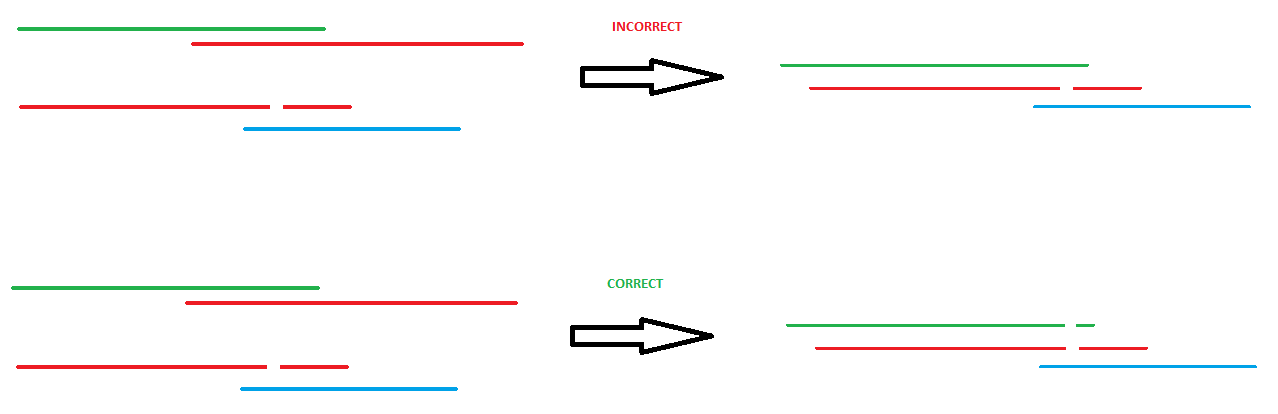
\includegraphics[scale =0.4]{images/gapPrecedent.png}
	\caption{\label{gapPrecedent}Exemple de propagation d'un gap vers les fragments précédents}
\end{figure}

\begin{figure}
\centering
	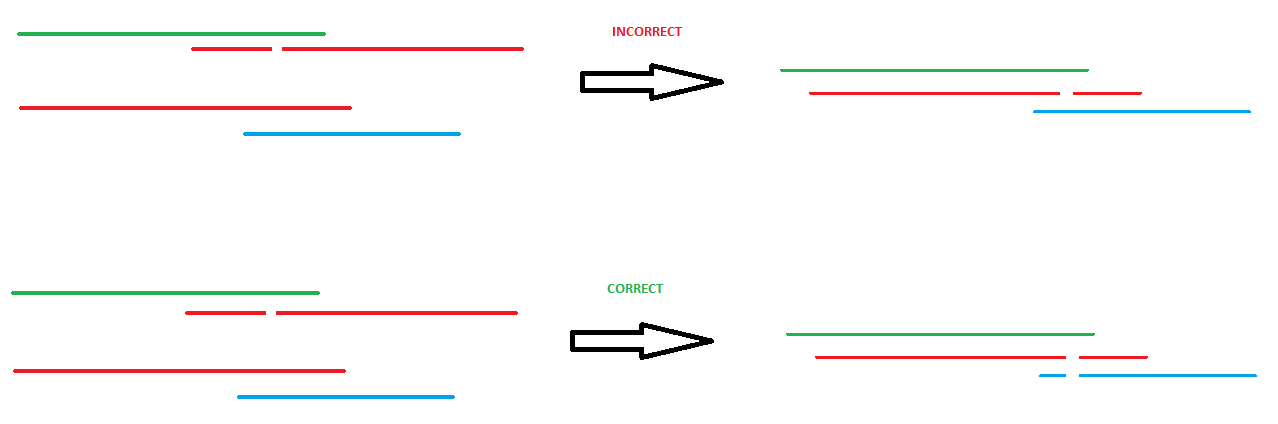
\includegraphics[scale =0.4]{images/gapSuivant.png}
	\caption{\label{gapSuivant}Exemple de propagation d'un gap vers les fragments futurs}
\end{figure}

\bibliographystyle{plain}
\bibliography{reference}

\end{document} 